\chapter{Original Work}
    \label{chp:ow}
    Finally, this Chapter is dedicated to the presentation and discussion of the original work and implementation of this research thesis. It is divided in four main sections. At first, Section \ref{ow:purposethesis} is concerned with the purpose of the research, which concepts, architectures and ideas have been borrowed from the State-of-the-Art research and references to previous chapters and sections are given. Section \ref{ow:beliefmodule} presents the original module, called Belief-Estimation module, in all its components, mechanisms and design choices, by detailing step-by-step the operations that are involved and the loss function upon which it is trained. Afterwards, Section \ref{ow:deterministic_module} is concerned with the presentation of an intermediate step of our research, the State-Prediction module, which represents a simpler but meaningful network developed during the research and that has been used as a baseline in Chapter \ref{chp:results}. At last, Section \ref{ow:application_sota} explains the range of applicability of the proposed Modules along with the actual implementation alongside a State-of-the-Art Reinforcement Learning algorithm, TRPO.
    
    \section{Original Implementation Objective}
    \label{ow:purposethesis}
        % Which of the State-of-the-Art topics have been used, when and why.
        %   - Delay Approaches: Model-Based Approach
        %   - POMDP Literature: Predictive-State Representation Approach
        %   - Deep Learning Literature: Attention Networks over Recurrent Networks
        The purpose of this thesis is to push forward the field of DMDP. As stated in the Introduction, the presence of delays does not represent a rare and particular case for MDP problem. Delays are present in the real world, they stem from many different sources, such as computational time or data transmission time, which are present exactly due to the physical implementation of the Agent. Thus, it is important to embed the presence of delays in the MDP framework, so to train agents that are capable to carry out a meaningful and precise decision-making process. However, literature specific to the DMDP framework is still scarce and wide-applicable solutions are yet to be found. \newline
        This thesis strive for the definition of a new implementation in the Model-Based approach for DMDP that is able to deal with both deterministic and stochastic delays in the context of both deterministic and stochastic environments. We would like to tackle the problem of delays with a heuristic approach: we provide to the RL algorithm either a prediction of the current state or a belief distribution of the current state. While the prediction of a state can be given explicitly, the belief distribution is handled out as a learnt vector representation. \newline
        Within this section, the design choices that lead to the definition of the Module's architecture are explained, detailing its structure in a step-by-step fashion in order to highlight how its design choices affected the final result. 
        
        \subsubsection{Assumptions of the Research}
            Before the presentation of the research development and results, it is important to highlight which assumptions and properties are taken. Throughout the rest of this chapter, the following statements and properties are assumed true:
            \begin{itemize}
                \setlength\itemsep{0.05em}
                \item Known delays: at each time-step, the Agent is aware of the amount of delay present, $d_t$, which is either constant or sampled from a stochastic process $d(t)$.
                \item Observation delays: we leverage the equivalency between observation delays and execution delays stated in Theorem \ref{th:dmdpred} by only referring to observation delays.
                \item Time-Discretization: we assume that the amount of delay at each time-step is a multiple of the time-step unit of the environment. This is ensured through the simulation of the delay implemented. Further details are given in Section \ref{sub:simulated_delays}.
            \end{itemize}
            At last, we mention the fact that not all component of the module and the environments are originally implemented. The entire research is coded in Python 3.7 and we referred to known and trusted libraries such as PyTorch (\pcite{python:pytorch}) for network layers implementation and OpenAI Gym (\pcite{python:gym}) for enviroments implementation and OpenAI SpinningUp (\pcite{python:spinningup}) for RL algorithm implementation.
            
        \subsection{Model-Based Approach}
            % Why Model-Based over Augmented and Memoryless
            In Section \ref{sota:delay_approaches}, three different approaches to the problem of delays are presented, each one with its own advantages and disadvantages. Among these three, Model-Based reveals to be the most flexible and applicable approach, giving room for experimenting different solutions for different environment and delay contexts.
            % - Design possibilities
            \subsubsection{Flexible Approach}
                The clear separation between the State Representation step and the Action Selection step, both presented in Section \ref{subs:modelbasedapproach}, allows for dividing the design process of a new architecture in two correspondent parts: what and how to compute from the available knowledge at each time-step, i.e. the extended state $i_t$; and how to deal with optimal action selection, upon whichever results is given by the first part. Our implementation is focused on solving the State Representation step, while the Action Selection step is solved through an existing RL algorithm, TRPO in our case. Both other two approaches do not offer this freedom of design choice.
                
            % - The concept of modularity and wide applicability
            \subsubsection{Range of Applicability}
                For the same reasons, Model-Based approach offers a wider and more direct applicability. Both Augmented and Memoryless are compatible with existing RL algorithm, as explained in Sections \ref{subs:augmentedapproach} and \ref{subs:memorylessapproach}. However, the first is also characterized by an exponential State Space $\mathbf{I_d}$, while the second requires ad-hoc solution to inject knowledge of delays. Both of them rely entirely on the network structure of the RL algorithm, which in general does not support variable-size inputs, thus it is unclear how to tackle stochastic delays. In contrast, Model-Based approach addresses all these aspects within the State Representation step, which outputs a state prediction or a belief representation of fixed-size. The deployed RL algorithm perceives the state predictions or belief representations as if they were the State Space $\mathbf{S}$, thus ensuring direct compatibility regardless of the kind of delay.
                
            % - The need of learning a model of the environment
            \subsubsection{Learning the Model of the Environment}
                At last, Model-Based approach offers the possibility of learning the model of the Environment with the network architecture that implements the State Representation step. The fact that the module has a specific, observable objective makes it easier to evaluate its performances, since we do not need to always deploy a RL algorithm, train the whole architecture and inspect the Agent's final performances. Each design choice can be implemented and tested directly on the module by comparing its performances with previous iterations, inspecting their loss functions, for example. This whole procedure do not affect the RL algorithm deployed, since they interact only through the module's output, thus allowing freedom of design choices.
                \\\\
            
            For these reasons, the proposed new Modules represent a new and original implementation of the State Representation step in the context of Model-Based approach for Delayed Reinforcement Learning problems. The Action Selection step is addressed by TRPO. Figure \ref{fig:module_modelbased_view} illustrates the entire architecture from the Model-Based approach point of view.
                
                \begin{figure}[!t]
                        \centering
                        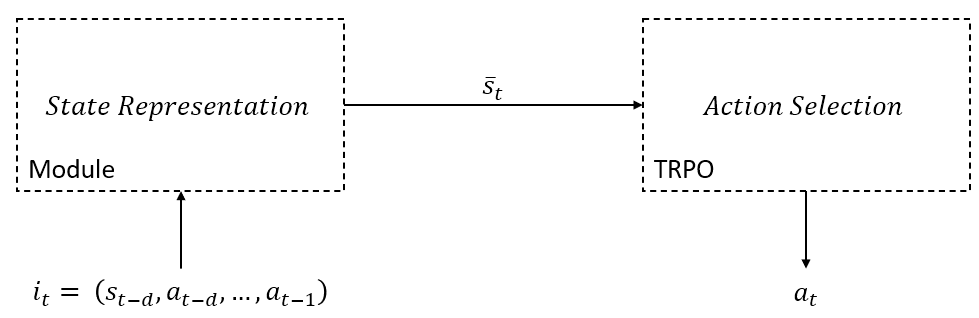
\includegraphics[width=15cm, keepaspectratio]{images/module/modelbased_view.png}
                        \caption{Model-Based approach view of the Modules architecture.}
                        \label{fig:module_modelbased_view}
                \end{figure}
            
        \subsection{Predictive-State Representation Approach}
            % What does the Module do in practice, which paradigms are applied
            Up until now, the original module has been pictured as a black box that implements the State Representation step in a Model-Based approach context. In order to further explain the details of the implementation, the main paradigm that leads the implementation must be defined. In this regard, POMDP literature have been useful to define the general approach. As explained in Section \ref{sota:pomdp}, DMDP framework is closely related to POMDP framework: DMDPs that are tackled with a Memoryless approach or by letting the Agent observe a belief can be formulated as a particular cases of POMDP where the knowledge available to the Agent represents the observation perceived from the Environment. Predictive-State Representation (PSR) is a successful paradigm exploited by POMDP algorithms that is closely related to the Model-Based approach for DMDPs. For this reason, it has been adopted for guiding the practical implementation of the original modules.
            
            % - Learning a State Representation 
            \subsubsection{State Representation Learning}
                As presented in Section \ref{subs:psd}, Predictive-State Representation is applicable to architectures or networks that are able to maintain an internal state $h$ in addition to the usual output $y$, from processing their input. While $y$ is used by the Policy function to carry out action selection, the internal state $h$ is used to predict an observable quantity, $\bar{s}_t$. In addition to the usual performance measure $J$ that evaluates the Agent's decision-making process, a second loss function is defined to evaluate the ability of predicting $\bar{s}_t$, comparing it to the observed quantity, either the exact state $s_t$ or its belief distribution, for example. The observability of the said quantity is a key property, since its information needs to be available to the Agent at training time. The rest of this section is dedicated to a parallel comparison between the PSR architecture and the new developed modules, with the purpose of further detailing how they function.
                \\\\
                % - Takes as input available knowledge (observation/extended state)
                At each time-step $t$, PSR implementations take as input the current observation $o_t$, while our modules take as input the correspondent quantity in the context of the DMDP framework: the extended state $i_t$. Infact, both the current observation $o_t$ and the extended state $i_t$ represent the most updated information the Agent has available at each time-step. \newline
                % - Maintain an internal state h_t to predict future observation/states upon which a new Loss function is defined
                In both cases, the input is used to maintain the internal state $h$ by updating it through a mechanism implemented, denoted by a function $f$:
                \begin{align*}
                    h_t &= f_{PSR}(h_{t-1}, o_t)\\
                    h_t &= f_{Module}(h_{t-1}, i_t)
                \end{align*}
                where $f$ can be a Recurrent mechanism, implemented by means of LSTM or GRU network, or an Attention mechanism. In the POMDP case, the internal state $h_t$ is then used to predict the sequence of next observations $\mathbf{s_t} = (o_{t+1}, o_{t+2}, ..., o_{t+d})$ through another component of the network, called encoder in \pcite{pomdp:psd} or through $\theta_{pred}$ in \pcite{pomdp:rpsp}, for example. In our modules, the internal state $h_t$ is used to predict the sequence of yet unobserved states of the environment $\mathbf{s_t} = (s_{t-d+1}, s_{t-d+2}, ..., s_t)$ or their belief distributions. This representes the main advantage of our modules against their POMDP counterparts: since the information about the sequence of the exact states visited in the trajectory is available at training time, although delayed, it is possible to predict them or their distribution. In turn, this allows for defining a predictive loss function $L$ upon exact quantities, rather than partial observations, which is able to drive the modules towards a more meaningful internal state w.r.t. their POMDP counterparts. \newline
                % - Output the prediction (y/knowledgeaboutcurrentposition)
                At last, the output $y$ is produced from the internal state $h$. In the POMDP case, the internal state $h$ is directly provided to the Policy network $\pi$ as input. In the DMDP case, our modules can be designed to handle out to the Policy network $\pi$ a quantity that is most suitable given the properties of the environment: the current state prediction in deterministic environments or the internal state $h_t$, trained to represent the belief distribution of the current unknown state, in stochastic environments.
                
            % - MultiTask Learning Algorithm
            \subsubsection{Multi-Task Learning}
                The adoption of the PSR paradigm for the Modules also implies that, when coupled with a Reinforcement Algorithm, the entire network becomes an instance of Multi-Task Learning (MTL). In practice, the modules can also be used in a stand-alone fashion for the purpose of predicting current information, whether the exact state or a belief distribution, about the Agent unknown state $s_t$. \newline
                This also allows for highlight the main advantage of the modular approach: since the training is separated from the rest of the network, they can be considered as an interface between the extended state $i_t$ and the state representation $\bar{s}_t$. This process is invisible to the RL algorithm deployed and as a consequence any RL algorithm can be deployed. Hence the name of modules to denote the proposed networks. Figure \ref{fig:module_psr_view} illustrates the entire architecture from the Predictive State Representation point of view.
                
            \begin{figure}[!t]
                        \centering
                        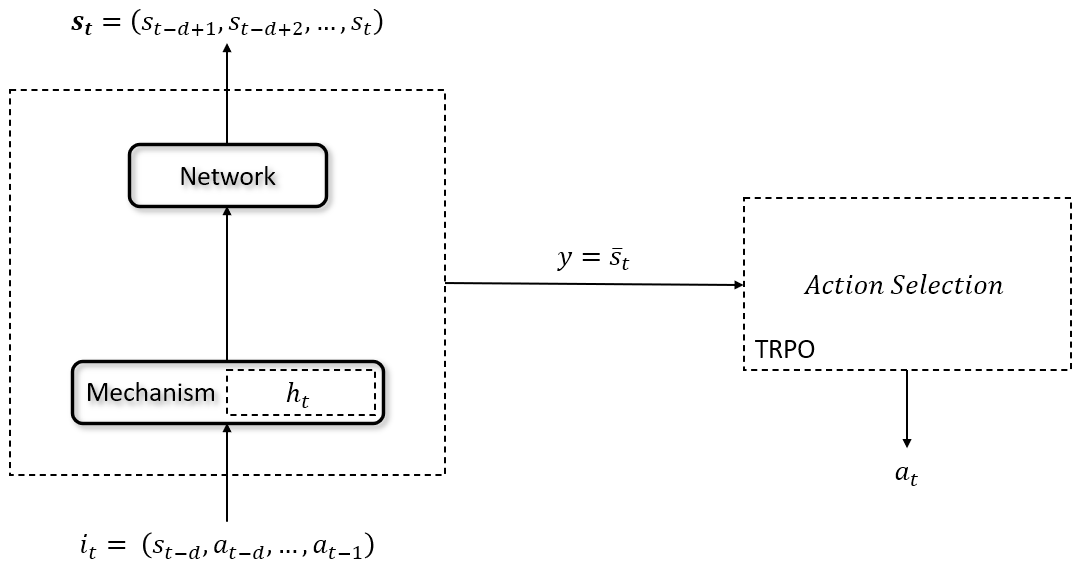
\includegraphics[width=15cm, keepaspectratio]{images/module/psr_view.png}
                        \caption{Predictive-State Representation view of the Modules architecture.}
                        \label{fig:module_psr_view}
            \end{figure}
            
        \subsection{Self-Attention Mechanism}
            % - The modular property comes with a cost: computing the prediction for each extended state
            The modular property explained in the previous section is one of the strengths of the design of the Module. However, it also comes with the cost of passing each single extended state $i_t$ also through the module. This means that the computational overhead the Module introduces w.r.t. the Reinforcement Learning algorithm it is coupled with grows linearly with the total number of samples the entire network is trained upon. In the context of Reinforcement Learning, the total number of samples can easily reach millions, as shown in Chapter \ref{chp:results}. Thus, having an efficient mechanism that is able to maintain a meaningful internal state is a strong requirement. Otherwise, the risk is to lose the advantage introduced by the module because of the tremendous computational complexity the overall network requires. \newline
            
            % - Sequence-to-Sequence Models
            \subsubsection{Sequence-to-sequence Model}
                The modules' task can be seen as a translation from the extended state $i_t = (s_{t-d}, a_{t-d}, ..., a_{t-1})$ to the sequence of either unobserved states $(s_{t-d+1}, s_{t-d+2}, ..., s_t)$ or their belief distribution, which means that it is possible to model it through a Sequence-to-sequence model. In practice, this means that Recurrent and Attention mechanisms can be exploited to implement and mantain the internal state $h$, as explained in Section \ref{sota:selfan}. Attention is the chosen mechanism, given the optimization complexity that Recurrent implies: non-convex optimization and a number of sequential step that strictly depends on the length of the sequences involved, which in this case is dictated by the length of the delay.
            
            \begin{figure}[!t]
                    \centering
                    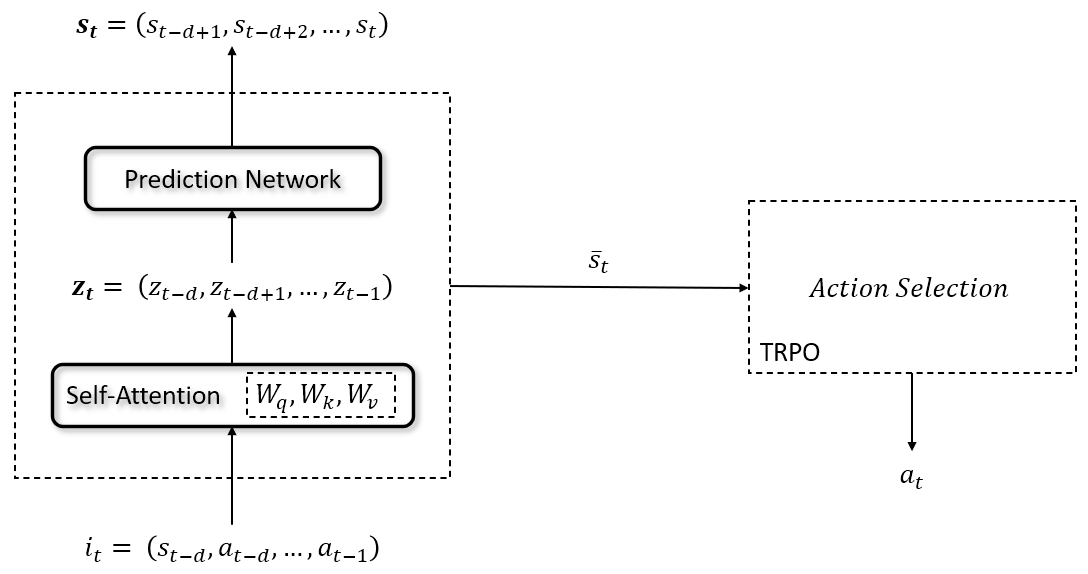
\includegraphics[width=15cm, keepaspectratio]{images/module/selfattention_view.png}
                    \caption{Self-Attention mechanism view of the Modules architecture.}
                    \label{fig:module_selfattention_view}
            \end{figure}
            
            % - Attention Mechanism provides a way to maintain a meaningful internal state, (W_q, W_k, W_v), also gives 
            \subsubsection{Self-Attention mechanism}
                In particular, Self-Attention provides a concrete implementation of the attention mechanism that is also free from Recurrent components while being able to compete with other state-of-the-art implementations, as illustrated in Section \ref{sub:transformer}. Thus the Modules' core components are represented by a sequence of Transformer's Encoder layers and a Prediction network. In practice, at each time-step $t$, the extended state $i_t$ is taken as input by the Self-Attention network, which produces the sequence of Attention vectors $\mathbf{z_t}$. Then, the Prediction network takes as input $\mathbf{z_t}$ and produces the state representation $\bar{s_t}$. The Prediction network remains generically defined at the moment because its structure depends on the Environment's properties. The two modules will present two different Prediction network, which will be described in their correspondent Sections. Figure \ref{fig:module_selfattention_view} illustrates the entire architecture from the Self-Attention mechanism point of view.
                
    
    \newpage
    \section{Belief-Estimation Module (Stochastic MDPs)}
        \label{ow:beliefmodule}
        % Introduction of the Belief-Estimation module
        In Section \ref{ow:purposethesis}, the overview of the module’s architecture is explained and illustrated. However, specific implementation details still need to be defined, along with the training and testing routine of the modules coupled with TRPO algorithm. \newline
        This section is dedicated to the Belief-Estimation module, designed to deal with stochastic environments, thus also supporting deterministic ones as a special case. Being able to cope with both deterministic and stochastic delays by construction, the Belief-Estimation module represents the final goal of this research thesis. In particular, we look for exploiting the Self-Attention mechanism provided by the Transformer's Encoders (Section \ref{sub:selfan}) to compute a fixed-length attention vector from a variable-length input sequence (Section \ref{sub:shape_input}), where the variability is present due to stochastic delays, which is then trained to represent the belief distribution of the current unobserved state through a MAF network (Section \ref{sub:maf_network}). At last, the belief representation is handled to a RL algorithm, TRPO in our case, in order to carry out action selection. The rest of the section is dedicated to present the sequence of components and operations that occur within them and to define the module's loss function.
        
        % Deterministic Module Structure:
        %   - From Extended State to (State, Action) couples (--> Words in NLT)
        \subsection{Shaping the Input}
            \label{sub:shape_input}
            The first issue encountered is the shape of the Module's input. Deciding to model the architecture as a Sequence-to-Sequence model means that the input shape must be a sequence, but the extended state $i_t = (s_{t-d}, a_{t-d}, ..., a_{t-1})$ does not immediately fit the needs. Infact, in Sequence-to-Sequence models each element of the sequence is an atomic element semantically equivalent to the others: in Neural Machine Translation, sequences are phrases and each element represents a word of the sequence, which are by definition equivalent to each other. In contrast, the extended state elements are not equivalent to each other: the first element is a state of the environment, while all the others are actions chosen by the Agent. In order to solve this issue, we decided to reshape the extended state in a sequence of couples $\mathbf{i_t}$ defined as follows:
            \[ i_t = (s_{t-d}, a_{t-d}, ..., a_{t-1}) \rightarrow \mathbf{i_t} =  \left[ (s_{t-d}, a_{t-d});  (s_{t-d}, a_{t-d+1}); ... ; (s_{t-d}, a_{t-1}) \right] \]
            Each couple $(s_{t-d}, a_{t-d+i})$ encapsulates the information of having observed state $s_{t-d}$ and decided to execute action $a_{t-d+i}$ a number of time-step $i$ later, with $0 \leq i \leq d - 1$. Also, reshaping makes each input element of the same size. This information is equivalent for each couple, exactly like words represents equivalent information in sentence.
            
        %   - Encoder (Transformer Architecture)
        \subsection{Self-Attention Network}
            \label{sub:selfan}
            After being reshaped into a sequence of couples, the input sequence is ready to be processed by the Self-Attention network. Similarly to the Transformer architecture, the main objective of this network is to produce a sequence of Attention vectors $\mathbf{z_t} = (z_{t-d}, z_{t-d+1}, ..., z_{t-1})$. Each Attention vector $z_{t-d+i}$, with $0 \leq i \leq d-1$, represents knowledge about the couple $(s_{t-d}, a_{t-d+i})$ and its correlation with the other couples according to the Self-Attention mechanism, explained in Section \ref{sub:transformer}. Infact, we believe that it is beneficial, if not crucial, to relate each couple to the others. In the undelayed MDP framework, each action selection is treated as independent from each other, thanks to the Markov Property (Property \ref{def:markov}). In the DMDP framework, this property does not hold for the sequence of actions chosen after the last observed state $s_{t-d}$. This means that looking only at the last observed states, thus considering each couple $(s_{t-d}, a_{t-d+i})$ independently from one another, is not sufficient to capture enough knowledge for a precise belief estimation.
            
            \subsubsection{Input Mapping}
        %       - Input Mapping (from Couples to intermediate representation --> Embedding in NLT)
                At first, each couple $(s_{t-d}, a_{t-d+i})$ of the input sequence $\mathbf{i_t}$ is translated through a Linear Input Mapping layer, which parameters needs to be learnt throughout the training process. In practice, each couple is treated as a vector and the following operation occurs in the Input Mapping layer:
                \[ x_{t-d+i} = ReLu \left( \theta_{input}^{T} * [s_{t-d}, a_{t-d+i}] + b_{input} \right)\]
                with $0 \leq i \leq d - 1$. The sequence of mapped couples is denoted by $\mathbf{x_t} = (x_{t-d}, x_{t-d+1}, $ $..., x_{t-1})$. This step of the process can be seen as an embedding of each couple, with the same conceptual meaning that Word Embedding holds in the case of Neural Machine Translation. Thus, the couples are translated from a vector of dimension $State Dimension + Action Dimension$ to a vector of dimension $enc_{dim}$, which represents an hyperparameter of the Module. At last, the result of the Input Mapping is passed through a ReLu activation function.
                \\\\
                Optionally, we inserted the possibility to rescale the couples before the Input Mapping takes place. Each element of each couple $(s_{t-d}, a_{t-d+i})$ is normalized in the interval $[-1,1]$. We believe this option is necessary because the couples vectors $(s_{t-d}, a_{t-d+i})$ holds elements with very different physical meaning: $s_{t-d}$ represents the state dimensions while $a_{t-d+i}$ represents the action dimensions, which means that, in general, they may assume values of different order of magnitude. Thus, rescaling them to match the same interval $[-1,1]$ avoids implicitly assigning a greater importance to dimensions that holds the largest values, as it would happen otherwise, due to numerical operations within the network. Whether rescaling the couples or not is an hyperparameter of the Module.
                
            \subsubsection{Positional Encoding}
        %       - Positional Encoding (Position in the sequence matters)
                As explained in Section \ref{sub:transformer}, the Transfomer architecture allows for encoding positional information within each element of the input sequence. Infact, as it happens for words in a sentence, the order and position of each elements matter, since the sequence of actions in the original extended state $i_t$ represents the sequence of decisions made by the Agent. Following Equation \ref{eq:pos_enc}, a vector $p_i$ encoding positional information is computed and added to each element of the input sequence $x_{t-d+i}$:
                
                \[ x_{t-d+i}^{pos} = x_{t-d+i} + p_i \]
                
                In order to correctly implement Positional Encoding, the hyperparameter $enc_{dim}$, which defines $x_{t-d+i}$ dimension in the Input Mapping, must be equal to $p_i$ dimension. For simplicity of notation, $x_{t-d+i}^{pos}$ will still be denoted by $x_{t-d+i}$.
                
            \subsubsection{Layer Normalization}
        %       - Layer Normalization
                After the Positional Encoding is embedded in the sequence $\mathbf{x_t}$, a Layer Normalization is used to normalize values of each element $x_{t-d+i}$. Following Equation \ref{eq:layer_norm}, the following computation is carried out on each element $x_{t-d+i}$:
                
                \[ x^{norm}_{t-d+i} = \frac{x_{t-d+i} - \mathbf{E} \left[ x_{t-d+i} \right]}{\sqrt{\mathbf{Var} \left[ x_{t-d+i} \right] + \epsilon}} * \gamma + \beta\]
                
                where $\mathbf{E} \left[ x_{t-d+i} \right]$ and $\mathbf{Var} \left[ x_{t-d+i} \right]$ are estimated element-wise on the input batch the module is supplied with at each training process; $\epsilon$ represents a low value for numerical stability, usually set to $10^{-5}$, while $\gamma$ and $\beta$ represents learnable parameters of the layer and thus for the module. Again, for simplicity of notation, $x^{norm}_{t-d+i}$ will still be denoted as $x_{t-d+i}$.
                
            \subsubsection{Causal Mask}
        %       - Optional: Causal Mask (True for Deteministic in our results)
                Before processing the sequence $\mathbf{x_t}$ through the Encoder layers, we adopt the Input Sequence Mask option, presented in seciton \ref{sub:transformer}, in order to embed temporal causality within the model. Thus, we construct a Causal mask to be supplied to the Encoder Layer's implementation. A Causal mask is a mask that zeroes out all elements' score that come after the currently processed element, thus letting it relate only to previous elements. \newline
                The idea behind the implementation of the causal mask is that each action in the extended state $i_t$, and thus each element in $\mathbf{x_t}$, is only dependent on the previous actions and not the following ones. Thus, avoiding to relate each element $x_{t-d+i}$ with the future ones may be beneficial for the overall performances. Whether applying the Causal mask or not is an hyperparameter of the Module.
                
            \subsubsection{Encoder Layers}
        %       - Encoder Layers
                After Normalization Layer, a Transformer Encoder is implemented in order to carry out the Attention mechanism in the Module. As explained in Section \ref{sub:transformer}, the Transformer Encoder stacks one or more Encoder layers sequentially. Each one of them takes as input either the sequence $\mathbf{x_t}$ or their previous layer' output sequence $\mathbf{z_{t}^{j}}$, where $j$ denotes the outputs of the $j$-th Encoder layer along with the Causal mask, if it is enabled for the module. Encoder layer's attention computation is not modified from the Transformer's original implementation. However, our Module is based on the PyTorch implementation of a Transformer Encoder layer and for the sake of completeness and precision, we report the sequence of computations implemented:
                
                \begin{itemize}
                \setlength\itemsep{0.05em}
                    \item Self-Attention Layer, as illustrated in Figure \ref{fig:an_transformer_encoder}:
                    \begin{itemize}
                        \setlength\itemsep{0.05em}
                        \item Self-Attention computation: as explained in Section \ref{sub:transformer};
                        \item Dropout;
                        \item Layer Normalization: as explained in Section \ref{sub:transformer};
                    \end{itemize}
                    \item Feedforward Layer, as illustrated in Figure \ref{fig:an_transformer_encoder}:
                    \begin{itemize}
                        \setlength\itemsep{0.05em}
                        \item Linear Layer: as explain at the beginning of this Section;
                        \item Activation Layer: the activation function ReLu has been chosen;
                        \item Dropout Layer;
                        \item Linear Layer: as explain at the beginning of this Section;
                        \item Dropout Layer;
                        \item Layer Normalization: as explained in Section \ref{sub:transformer};
                    \end{itemize}
                \end{itemize}
                
                where Linear layers and Layer Normalizations have been already explained previously. Dropout is a regularization technique proposed by \pcite{dl:dropout}, which consists in zeroing out some elements of the input sequence during training. It adds as hyperparameter of the Module the probability $p_{dropout}$ that an element of the input is zeroed during training. \newline
                The result obtained is the sequence of Attention vectors, $\mathbf{z_t} = (z_{t-d}, z_{t-d+1}, ..., z_{t-1})$, where each element contains the information regarding the correspondent $x_{t-d+i}$ element and its attention relation with other elements of $\mathbf{x_t}$. The number of Encoder layers $e$, the dimension of the encoder vectors $q$, $k$ and $v$, denoted as $enc_{dim}$ and the dimensions of the Feedforward layers $encff_{dim}$ represent hyperparameters of the Module.
                
            \subsubsection{Encoder Output Mapping}
        %       - Encoder Output Mapping (from Encoder Layers Dimension to Attention Vectors Dimension)
                The last step of the Self-Attention network is a Linear Output Mapping, which serves the purpose to match Attention vectors dimension $enc_{dim}$ to the dimension expected by the Prediction network, $pred_{dim}$. The computation is analogous to the Linear Input Mapping, for each element in the sequence $\mathbf{z_t}$:
                \[ z^{pred}_{t-d+i} = ReLu \left( \theta_{output}^{T} * z_{t-d+i} + b_{output} \right)\]
                where $\theta_{output}$ and $b_{output}$ represents learnable parameters and the dimension $pred_{dim}$ a hyperparameter of the State-Prediction Module. As it happened previously, the elements $z^{pred}_{t-d+i}$ will still be denoted as $z_{t-d+i}$ for simplicity of notation.
        
        % MAF Implementation as Prediction Network
        \subsection{Masked Autoregressive Flow Network}
            \label{sub:maf_network}
            As explained in Section \ref{prel:maf}, Masked Autoregressive Flow is a neural density estimation technique: it allows for estimating a conditional density $p(\mathbf{x}\vert\mathbf{y})$ given a set of examples $\{\mathbf{x}_n, \mathbf{y}_n \}$, where $n$ represents the number of total examples. Our objective is to use MAF network to estimate the density of the unobserved states $s_{t-d+i}$ conditioned on the extended state $i_t = (s_{t-d}, a_{t-d}, ..., a_{t-1})$, thus $p(s_{t-d+i} \vert i_t)$ with $1 \leq i \leq d$.
            \\\\
            In order to achieve our objective, we need to represent the learnt density $p_{pred}$ as a transformation by an invertible and differentiable function $f_{pred}$ of a base Gaussian density $q$. In practice, $f_{pred}$ is composed by a number of function couples $(f_{\mu_j}, f_{\alpha_j})$ equal to the state dimensions, denoted as $sdim$, since each couple is specifically tasked to build each dimension of the unobserved state $s_{t-d+i}$ as follows:
            
            \begin{align}
                s_{t-d+i}^{j} &= u_j e^{\alpha_j} + \mu_j\label{eq:beliefmod_normflow}\\
                \mu_j &\coloneqq f_{\mu_j} (\mathbf{u_{-j}}, z_{t-d+(i-1)})\nonumber\\
                \alpha_j &\coloneqq f_{\alpha_j}(\mathbf{u_{-j}}, z_{t-d+(i-1)})\nonumber
            \end{align}
           
            where $\mathbf{u} = (u_1, u_2, ..., u_{sdim}) \sim q$, its elements are denoted as $u_j$ and the subscript $-j$ denotes all elements in $\mathbf{u}$ before the $j$-th; $z_{t-d+(i-1)}$ is the Attention vector produced by the Self-Attention network correspondend to the state $s_{t-d+i}$, note that the additional -$1$ in the subscript is used to align the sequence of Attention vector $\mathbf{z_t}$ to the sequence of unobserved states. At last, the function couples $(f_{\mu_j}, f_{\alpha_j})$ are parametric functions, which parameters represents the set of learnable parameters of the MAF network. To be more specific w.r.t. the MAF original implementation, the set of equation and definitions \ref{eq:beliefmod_normflow} correspondes directly to the set of equations and definitions \ref{eq:maf_gauss_1} and \ref{eq:maf_gauss_2}. \newline
            In practice, we are conditioning density $p_{pred}$ by appending the Attention vectors $z_{t-d+(i-1)}$ produced by the Self-Attention network to the samples $\mathbf{u_{-j}}$ from the base density $q$, as explained in Section \ref{sub:maf}. This allows for expressing $p_{pred}$ through the following representation:
            \begin{align}
                \label{eq:beliefmod_ppred}
                p_{pred} (s_{t-d+i} \vert z_{t-d+(i-1)}) = q \left( f_{pred}^{-1} \left(s_{t-d+i}, z_{t-d+(i-1)} \right) \right) \abs*{det \left( \frac{\partial f_{pred}^{-1}}{\partial s_{t-d+i}} \right)}
            \end{align}
            which is a direct application of Equation \ref{eq:normflow}. Given the recursive nature of the network, which produces each state dimension at each recursion, the right-hand side determinant is easily computed, because $f_{pred}$'s Jacobian is a triangular matrix.
            
            % Explain how the Module is optimized --> Loss Function and Gradient-Based
            \subsubsection{Loss Function}
            Up to this point, we have explained how it is possible to compute the estimated density $p_{pred}$. To quickly recap, each extended state $i_t = (s_{t-d}, a_{t-d}, ..., a_{t-1})$ is first reshaped into couples $(s_{t-d}, a_{t-d+i})$ with $0 \leq i \leq d-1$. Each couple is then processed throughout the Self-Attention network, which produces the sequence of attention vectors $\mathbf{z_t} = (z_{t-d}, z_{t-d+1}, ..., z_{t-1})$. Each attention vector $z_{t-d+(i-1)}$ is then coupled with its correspondent unobserved state $s_{t-d+i}$, with $1 \leq i \leq d$ so to compute the conditional density $p_{pred} (s_{t-d+i} \vert z_{t-d+(i-1)})$ through Equation \ref{eq:beliefmod_ppred}. \newline
            Then Belief-Estimation module is thus trained upon the following loss function $L_{belief}$: 
            
            \begin{align}
                L_{belief}(\mathbf{z_{t}}, \mathbf{s_t}) \coloneqq \sum_{i}^{d} D_{KL} \left( p(s_{t-d+i} \vert i_t) || p_{pred}(s_{t-d+i} \vert z_{t-d+(i-1)}) \right)
            \end{align}
            
            where $\mathbf{s_t}$ is the sequence of unobserved states related to the extended state $i_t$ and $D_{KL}$ represents the Kullback-Leibler divergence. A replay buffer is implemented to retrieve a set of samples to compute $L_{belief}$, details are given in Section \ref{sub:dtrpo_buffers}. In practice, $L_{belief}$ computes the distance between the true state distribution conditioned on the extended state $i_t$ and the predicted state distribution conditioned on the attention vectors $\mathbf{z_t}$. The idea behind this design decision is that we would like to enforce the attention vectors to comprise all the available knowledge about the Agent's current, but unobserved, position by driving it towards a finite vector representation of the current belief distributionm which is then handled out to the RL algorithm, as a State Representation according to the Model-based approach. Hence the name of the module: Belief-Estimation module. \newline
            For the actual implementation, $L_{belief}$ is substituted by using the following log-likelihood approximation:
            
            \begin{align}
                L_{belief}(\mathbf{z_t}, \mathbf{s_t}) \coloneqq \sum_{i=1}^{d} \log p_{pred} \left(s_{t-d+i} \vert z_{t-d+(i-1)} \right)
            \end{align}
            
            By construction, $p_{pred}$ is differentiable w.r.t. its set of learnable parameters, thus we can exploit any gradient-based optimization algorithm to optimize the entire network. In practice, we exploited two different instances of the ADAM optimization algorithm: the first optimizes the Self-Attention network parameters, while the second optimizes the MAF network parameters.
        
    \newpage
    \section{State-Prediction Module}
    \label{ow:deterministic_module}
        During the development of the research, we focused first on deterministic environments given their reduced complexity w.r.t. stochastic environments, in order to test our approach. Thus, before the complete definition of the Belief-Estimation module was reached, we developed an intermediate result, designed to solve the delay problem in deterministic environments: the State-Prediction module. Its structure is similar to the final design, infact it exploits the same input shaping process (Section \ref{sub:shape_input}) and Self-Attention network (Section \ref{sub:selfan}). However, instead of providing a belief estimation through a MAF network, it provides a direct prediction of the current, unobserved Agent's position through a Linear layer, while the entire network is trained upon a mean-squared error loss, or L2 loss, computed between the state prediction $\tilde{s}_t$ and the observed delayed state $s_t$. The state prediction is then handled out to the RL algorithm. This section is dedicated to detailing the Prediction network.
        
        \subsection{Prediction Network}
        \label{sub:pred_network}
        %   - Output Mapping (from Attention Vectors to Predicted States)
            As introduced, the last step of the State-Prediction Module is concerned with deriving the sequence of state prediction $\mathbf{s_t}$ from the sequence of Attention vectors $\mathbf{z_t}$. A Linear layer is implemented for the task and the computation is analogous to the one previously presented:
            
            \[ \tilde{s}_{t-d+i+1} = ReLu \left( \theta_{pred}^{T} * z_{t-d+i} + b_{pred} \right)\]
            
            where $\theta_{pred}$ and $b_{pred}$ are learnable parameter for the Module. Note that the dimension of the output vectors $\tilde{s}_{t-d+i+1}$ is not a parameter, since it is the state dimension, dictated by the Environment. We denote by $\mathbf{\tilde{s}_t} = (\tilde{s}_{t-d+1}, \tilde{s}_{t-d+2}, ..., \tilde{s}_t)$ the output sequence of the State-Prediction module. 
            \\\\
            At last, it is important to specify that in the case of rescaling the input during the Input Mapping explained in the previous section, the output could be rescaled back to match the actual state dimensions values, by multiplying each dimension for the scaling factor used at the beginning. 
            
            % Explain how the Module is optimized --> Loss Function and Gradient-Based
            \subsubsection{Loss Function}
                Now that the output sequence of the module has been defined, it is also possible to specify how the State Prediction module is optimized. We define a mean-squared error loss function, denoted as $L_{pred}$, over the output sequence $\mathbf{\tilde{s}_t}$ and the sequence of actually, delayed observed states $\mathbf{s_t} = (s_{t-d+1}, s_{t-d+2}, ..., s_t)$:
                \begin{align}
                    L_{pred} (\mathbf{\tilde{s}_t}, \mathbf{s_t}) \coloneqq \frac{1}{d} \sum_{i}^{d} \left( s_{t-d+i} - \tilde{s}_{t-d+i}\right)^{2}
                \end{align}
                after which any gradient based optimization algorithm can be exploited to update the module's parameters, since by construction the State-Prediction module is differentiable w.r.t. its set of learnable parameters. We decided to exploit ADAM, an algorithm for first-order gradient-based optimization proposed by \pcite{opt:adam}, to optimize the module. A replay buffer is implemented to retrieve a set of samples to compute $L_{pred}$, details are given in Section \ref{sub:dtrpo_buffers}. In practice, by optimizing the State-Prediction odule using $L_{pred}$, we drive the entire network towards the prediction of the current, unobserved state, which is handled out to the RL algorithm as a State Representation according to the Model-based approach. Hence the name of the module: State-Prediction Module.
    
    \newpage
    \section{Applications with State of the Art Algorithms}
    \label{ow:application_sota}
        % Introduction:
        %   - Seq2Seq usually trained in ML context (data set)...
        %   - ...we needed a RL context (trajectories)
        %   - Thus Module trained along with Policies/Values
        %   - Thus a Prediction Buffer 
        In the previous sections, both modules have been presented along with their loss functions, which they are trained upon. At this point, it is important to define the details about its deployment: the module training procedure and its interaction with the RL algorithm. In this section, we first describe the training procedure of the module (Section \ref{sub:dtrpo_buffers}) and then we detail the implemented application alongside TRPO algorithm (Section \ref{sub:dtrpo}).
        
        % Training Loop in RL + Prediction Buffers
        \subsection{Training and Prediction Buffers}
        \label{sub:dtrpo_buffers}
            The main issue in designing the training procedure is concerned with the fact that, usually, Sequence-to-sequence models training is based on a fixed dataset of examples the model is trained upon, while RL algorithms rely on drawing a certain number of new trajectories at each epoch, which are then used to update its policy and value functions. Given the policy and value function updates, the distribution of the trajectories $p_{\tau}$ is not stationary through the epochs and it may change considerably: the final purpose is to retrieve an optimal policy, which will draw trajectories that are very different from the initial, randomly initialized, policy.
            The fact that the trajectory distribution $p_{\tau}$ is not stationary during training poses serious constraints on the training procedure:
            \begin{itemize}
                \setlength\itemsep{0.05em}
                \item While it is feasible to gather an unlimited number of trajectories before training policy and value function, thus building a dataset of state representation $\bar{s}_t$, computed from the extended states observed, and correspondent unobserved states $s_t$, the policy function that would drawn them is necessarily a randomly initialized one. Thus, in general, the policy would not be able to properly explore the environment and the built dataset cannot be considered reliable. In practice, we expect the module's performances to decrease whenever the policy starts drawing trajectories that visits new extended states w.r.t. the ones used to build the datasets.
                \item At the same time, training the module upon the state representations $\bar{s}_t$ resulting from set of extended states visited at each epoch can be a limiting factor. The module would learn upon a different trajectory distribution at each epoch, thus potentially creating instability during the module's updates. In turn, the policy would be affected by a low quality state or belief representations as input.
            \end{itemize}
            \noindent
            In order to design a robust training algorithm for the modules, we need to find a middle-ground between this two extremes approaches.
            
            \subsubsection{Prediction Buffer}
                We decided to implement a Replay Buffer for the module, called Prediction Buffer. The Prediction Buffer allows for storing experienced trajectories: at each time-step $t$, the current extended state $i_t$ and the state contained in it, $s_{t-d}$ are stored in the Prediction Buffer. Due to delay presence, the two stored vectors are disaligned time-wise: the currently observed extended state $i_t$ is used to produce $\bar{s}_t$, but provides the exact visited state $s_{t-d}$, which refers to $\bar{s}_{t-d}$. Thus, the Prediction Buffer implementation needs to be able to handle the re-alignment between them. At the end of each epoch, the Prediction Buffer is sampled: the sequence of extended states selected are used to produce their correspondent state or belief predictions $\bar{s}_t$ and along with the sequence of selected visited states $s_t$ they are used to compute the loss function.
                \\\\
                Due to the re-alignment procedure, two different Prediction Buffers are implemented. The first is tasked with handling deterministic delays, which presents a fixed-length disalignment between $i_t$ and $s_{t-d}$, and it is denoted as Deterministic Prediction Buffer. The second is developed to specifically handle the presence of stochastic delays, hence denoted as Stochastic Prediction Buffer. As explained in Section \ref{sub:dmdp_stochdelays}, the presence of stochastic delays creates a complex interaction between the Agent and the environment, where the time disalignment between $\bar{s}_t$ and $s_t$ is not fixed and the sequence of experienced states may not follow the same order of the visited states. Thus, a separate implementation have been developed to specifically handle this situations. Thanks to the known delays assumption, both Prediction Buffer are aware of the amount of delay at each time-step, which makes the re-alignment task feasible.
                \\\\
                Prediction Buffers are characterized by their size, i.e. the number of samples it can contain, and by their batch size, i.e. the number of samples that are used to train the module at the end of each epoch. Whenever the Prediction Buffer is full, older samples are removed in favor of the newer ones. Both size and batch size are considered hyperparameters of the module, given their impact in the learning process. As a result, the module is trained with experience replay, learning upon both new and old samples in order to smooth the trajectory distribution changes throughout the epochs with the purpose of stabilize the training process, overcoming the two critical issue described above.
                
        \subsection{Delay Trust Region Policy Optimization}
        \label{sub:dtrpo}
            
            % Better Explain the interaction between Modules and TRPO
            We decided to deploy both modules alongside TRPO algorithm, defining two variants of the same algorithm. We refer to the State-Prediction module deployment as L2-TRPO, given the nature of its loss function, while the Belief-Estimation module deployment has been called Delay TRPO or D-TRPO, in light of the fact that it represents our goal implementation. In practice, the modules presence is invisible to TRPO, which action selection is carried out unaltered from the original implementation upon a state space provided by the module. Thus, policy and value functions updates are implemented following Algorithm \ref{algo:trpo} specifications. Algorithm \ref{algo:dtrpo_l2trpo} illustrates both L2-TRPO and D-TRPO complete training algorithm: the differences between the two algorithms are contained within the module update and its Prediction Buffer routine. \newline
            At last, we present the options implemented within L2-TRPO and D-TRPO designed to optimize the training procedure of the algorithms, allowing for a better computational trade-off between the modules and the other two networks.
            
            \subsubsection{Pre-train Epochs}
            %   - Pretrain option for the Module
                Given the fact that all networks are randomly initialized at the start of the training process, the first epochs of training are characterized by low quality state or belief representation, which distribution is rapidly changing due to the gradient-based optimization method. As a consequence, policy and value networks updates during this first part of the training process are based on low quality information about the current position of the Agent in the environment, regardless of the type of module used and amount of delay present: the direction of optimization taken by their parameter vectors is not well-defined until the module is able to produce a better quality predictions. \newline
                In order to avoid wasting computational time and potentially lower the training quality of policy and value function, we believe it is useful to also have a way to decide to pre-train the module for a certain number of epochs before starting the Agent's training. We call this epochs Pre-train epochs and we consider the amount of pre-train epoch a hyperparameters of the algorithm, to be decided along the usual total number of training epochs. This allows for policy and value functions to be trained already upon meaningful state or belief representations.
                
            \subsubsection{Stopping the Module Training}
            %   - Stoptrain option for the Module
                On the other hand, it may be possible that the module is able to learn meaningful state or belief representation before the end of the whole training process. If this happens, continuing to update the module would be a waste of time and computational resources, which could re-directed towards the policy and value function networks: the same time spent updating the module could be instead used to update the other two networks for longer. At the same time, given the fact that the module is not updated anymore, its belief representation does not change over time and thus neither its distribution. Distribution changes in the input for the policy and value networks can be a source of instability in the learning process, which is avoided during this last epochs of training, resulting in more robust updates. \newline
                For this reason, we inserted the possibility to choose at which epoch the module's training is stopped, which is considered a hyperparameter of the trianing algorithm and it needs to be decided along with the total number of epochs and the number of pretrain epochs.
                
                \begin{algorithm}[t]
                    \SetAlgoLined
                    \DontPrintSemicolon
                    \KwResult{Optimal Policy $\pi_{\theta^*}$, Optimal Module $mod_{\varepsilon^*}$}
                    Initialize module $mod$ parameters, $\varepsilon_0$ randomly and its hyperparameters\;
                    Initialize policy $\pi$ parameters, $\theta_0$\;
                    Initialize value function $v$ parameters, $\phi_0$\;
                    Initialize Prediction Buffer $size$ and $batch$\;
                    Initialize TRPO hyperparameters\;
                    Initialize number of training epochs $E$, the number of pre-train epochs $P_e$ and the stop epoch $S_e$\;
                    Set the maximum number of steps of each epoch $T$\;
                    \While{$e \leq E$}{
                        Set current time-step $t=0$\;
                        Initialize the environment, retrieving the first extended state, $i_0$\;
                        \While{$t \leq T$}{
                            Compute the current State/Belief Representation $\bar{s}_t = mod_{\varepsilon}(i_t)$\;
                            Select action $a_t = \pi_{\theta} (\bar{s}_t)$\;
                            Observe the next extended state $i_{t+1}$\;
                            Receive the reward signal $r_t$\;
                            Store current information in the Prediction Buffer:\;
                            \ \ \ \ \ Extract $s_{t-d}$ from extended state $i_t$\;
                            \ \ \ \ \ Store $s_{t-d}$ and $i_t$\;
                            \ \ \ \ \ Align $s_{t-d}$ with $i_{t-d}$\;
                            Update time-step $t=t+1$\;
                            \If{Episode is terminated}{
                                Initialize the environment, retrieving the first extended state, $i_{t+2}$\;
                                Update time-step $t=t+1$\;
                            }
                        }
                        \If{$e \leq S_e$}{
                            Update module $mod$ parameters, $\varepsilon_e$:\;
                            \ \ \ \ \ Sample the Prediction Buffer: $\{s_t, i_t\}_{batch}$\;
                            \ \ \ \ \ Compute $\bar{s}_t$ for each $i_t$: $\{s_t, \bar{s}_t\}_{batch}$\;
                            \ \ \ \ \ Compute the Loss Function $L_{pred}$/$L_{belief}$ using $\{s_t, \bar{s}_t \}_{batch}$\;
                            \ \ \ \ \ Optimize the module via ADAM algorithm\;
                        }
                        \If{$e \geq P_e$}{
                            Update policy $\pi$ parameters, $\theta_e$, via TRPO algorithm\;
                            Update value function $v$ parameters, $\phi_e$, via TRPO algorithm\;
                        }
                    }
                    \caption{D-TRPO and L2-TRPO Training Algorithms.}
                    \label{algo:dtrpo_l2trpo}
                \end{algorithm}
        